% Options for packages loaded elsewhere
\PassOptionsToPackage{unicode}{hyperref}
\PassOptionsToPackage{hyphens}{url}
\documentclass[
  ignorenonframetext,
  aspectratio=169,
]{beamer}
\newif\ifbibliography
\usepackage{pgfpages}
\setbeamertemplate{caption}[numbered]
\setbeamertemplate{caption label separator}{: }
\setbeamercolor{caption name}{fg=normal text.fg}
\beamertemplatenavigationsymbolsempty
% remove section numbering
\setbeamertemplate{part page}{
  \centering
  \begin{beamercolorbox}[sep=16pt,center]{part title}
    \usebeamerfont{part title}\insertpart\par
  \end{beamercolorbox}
}
\setbeamertemplate{section page}{
  \centering
  \begin{beamercolorbox}[sep=12pt,center]{section title}
    \usebeamerfont{section title}\insertsection\par
  \end{beamercolorbox}
}
\setbeamertemplate{subsection page}{
  \centering
  \begin{beamercolorbox}[sep=8pt,center]{subsection title}
    \usebeamerfont{subsection title}\insertsubsection\par
  \end{beamercolorbox}
}
% Prevent slide breaks in the middle of a paragraph
\widowpenalties 1 10000
\raggedbottom
\AtBeginPart{
  \frame{\partpage}
}
\AtBeginSection{
  \ifbibliography
  \else
    \frame{\sectionpage}
  \fi
}
\AtBeginSubsection{
  \frame{\subsectionpage}
}
\usepackage{iftex}
\ifPDFTeX
  \usepackage[T1]{fontenc}
  \usepackage[utf8]{inputenc}
  \usepackage{textcomp} % provide euro and other symbols
\else % if luatex or xetex
  \usepackage{unicode-math} % this also loads fontspec
  \defaultfontfeatures{Scale=MatchLowercase}
  \defaultfontfeatures[\rmfamily]{Ligatures=TeX,Scale=1}
\fi
\usepackage{lmodern}
\usetheme[]{Boadilla}
\usefonttheme[]{professionalfonts}
\ifPDFTeX\else
  % xetex/luatex font selection
\fi
% Use upquote if available, for straight quotes in verbatim environments
\IfFileExists{upquote.sty}{\usepackage{upquote}}{}
\IfFileExists{microtype.sty}{% use microtype if available
  \usepackage[]{microtype}
  \UseMicrotypeSet[protrusion]{basicmath} % disable protrusion for tt fonts
}{}
\makeatletter
\@ifundefined{KOMAClassName}{% if non-KOMA class
  \IfFileExists{parskip.sty}{%
    \usepackage{parskip}
  }{% else
    \setlength{\parindent}{0pt}
    \setlength{\parskip}{6pt plus 2pt minus 1pt}}
}{% if KOMA class
  \KOMAoptions{parskip=half}}
\makeatother
\usepackage{graphicx}
\makeatletter
\newsavebox\pandoc@box
\newcommand*\pandocbounded[1]{% scales image to fit in text height/width
  \sbox\pandoc@box{#1}%
  \Gscale@div\@tempa{\textheight}{\dimexpr\ht\pandoc@box+\dp\pandoc@box\relax}%
  \Gscale@div\@tempb{\linewidth}{\wd\pandoc@box}%
  \ifdim\@tempb\p@<\@tempa\p@\let\@tempa\@tempb\fi% select the smaller of both
  \ifdim\@tempa\p@<\p@\scalebox{\@tempa}{\usebox\pandoc@box}%
  \else\usebox{\pandoc@box}%
  \fi%
}
% Set default figure placement to htbp
\def\fps@figure{htbp}
\makeatother
\setlength{\emergencystretch}{3em} % prevent overfull lines
\providecommand{\tightlist}{%
  \setlength{\itemsep}{0pt}\setlength{\parskip}{0pt}}
\usepackage[]{biblatex}
\addbibresource{bibliography.bib}
\usepackage{bm}
\usepackage{dsfont}
\usepackage{amssymb}
\usepackage{accents}
\usepackage[T2A,T1]{fontenc}


% bold letters (vectors)
\newcommand{\bnull}{\bm{0}}
\newcommand{\ba}{\bm{a}}
\newcommand{\bb}{\bm{b}}
\newcommand{\bc}{\bm{c}}
\newcommand{\bd}{\bm{d}}
\newcommand{\be}{\bm{e}}
% \newcommand{\bf}{\bm{f}}
\newcommand{\bg}{\bm{g}}
\newcommand{\bh}{\bm{h}}
\newcommand{\bi}{\bm{i}}
\newcommand{\bj}{\bm{j}}
\newcommand{\bk}{\bm{k}}
\newcommand{\bl}{\bm{l}}
% \newcommand{\bm}{\bm{m}}
\newcommand{\bn}{\bm{n}}
\newcommand{\bo}{\bm{o}}
\newcommand{\bp}{\bm{p}}
\newcommand{\bq}{\bm{q}}
\newcommand{\br}{\bm{r}}
\newcommand{\bs}{\bm{s}}
\newcommand{\bt}{\bm{t}}
\newcommand{\bu}{\bm{u}}
\newcommand{\bv}{\bm{v}}
\newcommand{\bw}{\bm{w}}
\newcommand{\bx}{\bm{x}}
\newcommand{\by}{\bm{y}}
\newcommand{\bz}{\bm{z}}

% bold letters (matrices)
\newcommand{\bA}{\bm{A}}
\newcommand{\bB}{\bm{B}}
\newcommand{\bC}{\bm{C}}
\newcommand{\bD}{\bm{D}}
\newcommand{\bE}{\bm{E}}
% \newcommand{\bf}{\bm{f}}
\newcommand{\bG}{\bm{G}}
\newcommand{\bH}{\bm{H}}
\newcommand{\bI}{\bm{I}}
\newcommand{\bJ}{\bm{J}}
\newcommand{\bK}{\bm{K}}
\newcommand{\bL}{\bm{L}}
\newcommand{\bM}{\bm{M}}
\newcommand{\bN}{\bm{N}}
\newcommand{\bO}{\bm{O}}
\newcommand{\bP}{\bm{P}}
\newcommand{\bQ}{\bm{Q}}
\newcommand{\bR}{\bm{R}}
\newcommand{\bS}{\bm{S}}
\newcommand{\bT}{\bm{T}}
\newcommand{\bU}{\bm{U}}
\newcommand{\bV}{\bm{V}}
\newcommand{\bW}{\bm{W}}
\newcommand{\bX}{\bm{X}}
\newcommand{\bY}{\bm{Y}}
\newcommand{\hbY}{\hat{\bm{Y}}}
\newcommand{\bZ}{\bm{Z}}


% calligraphic letters
\newcommand{\Acal}{\mathcal{A}}
\newcommand{\Bcal}{\mathcal{B}}
\newcommand{\Ccal}{\mathcal{C}}
\newcommand{\Dcal}{\mathcal{D}}
\newcommand{\Ecal}{\mathcal{E}}
\newcommand{\Fcal}{\mathcal{F}}
\newcommand{\Gcal}{\mathcal{G}}
\newcommand{\Hcal}{\mathcal{H}}
\newcommand{\Ical}{\mathcal{I}}
\newcommand{\Jcal}{\mathcal{J}}
\newcommand{\Kcal}{\mathcal{K}}
\newcommand{\Lcal}{\mathcal{L}}
\newcommand{\Mcal}{\mathcal{M}}
\newcommand{\Ncal}{\mathcal{N}}
\newcommand{\Ocal}{\mathcal{O}}
\newcommand{\Pcal}{\mathcal{P}}
\newcommand{\Qcal}{\mathcal{Q}}
\newcommand{\Rcal}{\mathcal{R}}
\newcommand{\Scal}{\mathcal{S}}
\newcommand{\Tcal}{\mathcal{T}}
\newcommand{\Ucal}{\mathcal{U}}
\newcommand{\Vcal}{\mathcal{V}}
\newcommand{\Wcal}{\mathcal{W}}
\newcommand{\Xcal}{\mathcal{X}}
\newcommand{\Ycal}{\mathcal{Y}}
\newcommand{\Zcal}{\mathcal{Z}}

% greek letters
\newcommand{\eps}{\varepsilon}
\newcommand{\sd}{\sigma}
\newcommand{\ssd}{\sigma^2}
\newcommand{\Sd}{\Sigma}
\newcommand{\Sdi}{\Sigma^{-1}}

\newcommand{\gb}[1]{\beta_#1}
\newcommand{\hbe}[1]{\hat{\beta}_#1}
\newcommand{\beps}{\bm{\varepsilon}}
\newcommand{\hbeps}{\hat{\bm{\varepsilon}}}

\newcommand{\balpha}{\bm{\alpha}}
\newcommand{\bbeta}{\bm{\beta}}
\newcommand{\hbbeta}{\hat{\bm{\beta}}}
\newcommand{\hssd}{\hat{\sigma^2}}
\newcommand{\bchi}{\bm{\chi}}
\newcommand{\bdelta}{\bm{\delta}}
\newcommand{\bepsilon}{\bm{\epsilon}}
\newcommand{\bphi}{\bm{\phi}}
\newcommand{\bgamma}{\bm{\gamma}}
\newcommand{\betah}{\bm{\etah}}
\newcommand{\bpi}{\bm{\pi}}


% prior and posterior parameters
\DeclareSymbolFont{cyrhelper}{T2A}{\familydefault}{m}{n}
\DeclareMathAccent{\post}{\mathord}{cyrhelper}{18}


\newcommand{\btheta}{\bm{\theta}}
\newcommand{\hbtheta}{\hat{\bm{\theta}}}

\newcommand{\thetapri}{\breve{\bm{\theta}}}
\newcommand{\thetapo}{\post{\bm{\theta}}}
\newcommand{\mupri}{\breve{\bm{\mu}}}
\newcommand{\mupo}{\post{\bm{\mu}}}
\newcommand{\Sdpri}{\breve{\Sigma}}
\newcommand{\Sdpo}{\post{\Sigma}}
\newcommand{\Sdipri}{\breve{\Sigma}^{-1}}
\newcommand{\Sdipo}{\post{\Sigma}^{-1}}

\newcommand{\apri}{\breve{a}}
\newcommand{\apo}{\post{a}}
\newcommand{\bpri}{\breve{b}}
\newcommand{\bpo}{\post{b}}

\newcommand{\btaus}{\bm{\tau}^2}
\newcommand{\taus}{\tau^2}


% other
\newcommand{\ty}{\tilde{\bm{y}}}
\newcommand{\tX}{\tilde{\bm{X}}}


\renewcommand{\bar}{\overline}


% statistics
\providecommand{\Pr}{}
\renewcommand{\Pr}{\mathbb{P}}
\newcommand{\Ex}{\mathbb{E}}
\newcommand{\var}{{\mathds{V}\mathrm{ar}}}
\newcommand{\cov}{{\mathds{C}\mathrm{ov}}}
\newcommand{\corr}{{\mathrm{Corr}}}
\newcommand{\ov}{\overline}
\newcommand{\wh}[1]{\widehat{#1}}
\newcommand{\wt}[1]{\widetilde{#1}}
\newcommand{\Cov}{\text{Cov}}
\newcommand{\IG}{\text{IG}}

\newcommand{\sumin}{\sum_{i = 1}^n}
\newcommand{\sumjn}{\sum_{j = 1}^n}
\definecolor{lmugreen}{RGB}{0,136,58}
\setbeamercolor{structure}{fg=lmugreen}
\usecolortheme[named=lmugreen]{structure}
\beamertemplatenavigationsymbolsempty
\usefonttheme{professionalfonts}
\usepackage{listings}
\lstset{
  language=R,
  basicstyle=\scriptsize\ttfamily,
  commentstyle=\ttfamily\color{gray},
  backgroundcolor=\color{white},
  showspaces=false,
  showstringspaces=false,
  showtabs=false,
  tabsize=2,
  captionpos=b,
  breaklines=false,
  breakatwhitespace=false,
  title=\lstname,
  escapeinside={},
  keywordstyle={},
  morekeywords={},
  belowskip=-1.2\baselineskip
}
\usepackage{caption}
\DeclareCaptionFont{tiny}{\tiny}
\captionsetup{font=scriptsize,labelfont=scriptsize,justification=centering}
\usepackage{textpos}
\addtobeamertemplate{frametitle}{}{%
  \begin{textblock*}{100mm}(0.88\textwidth,-0.5cm)
    
\includegraphics[height=1cm,width=2cm]{lmu_logo}
  \end{textblock*}}
\AtBeginSection[]{%
  \begin{frame}[noframenumbering,plain]%
    \frametitle{Outline}%
    \setcounter{tocdepth}{1}%
    \tableofcontents[currentsection]%
  \end{frame}}
\AtBeginEnvironment{thebibliography}{\scriptsize}
\usepackage{bookmark}
\IfFileExists{xurl.sty}{\usepackage{xurl}}{} % add URL line breaks if available
\urlstyle{same}
\hypersetup{
  pdftitle={Bayesianische Regression},
  pdfauthor={Lona Koers},
  hidelinks,
  pdfcreator={LaTeX via pandoc}}

\title{Bayesianische Regression}
\subtitle{lineare und logistische Modelle}
\author{Lona Koers}
\date{25. Juli 2025}
\institute{LMU}

\begin{document}
\frame{\titlepage}

\begin{frame}{Motivation und Intuition}
\protect\phantomsection\label{motivation-und-intuition}
TODO: gutes Intro-Beispiel

\begin{itemize}
\item
  Generalisierte Lineare Modelle (GLMs)
\item
  Punktvorhersage vs.~Verteilung vorhersagen
\item
  warum reicht uns ein CI / PI
\end{itemize}
\end{frame}

\section{\texorpdfstring{Bayesianisches \textbf{lineares} Modell
(LM)}{Bayesianisches lineares Modell (LM)}}\label{bayesianisches-lineares-modell-lm}

\begin{frame}{Frequentistisches \(\to\) bayesianisches lineares Modell}
\protect\phantomsection\label{frequentistisches-to-bayesianisches-lineares-modell}
Annahmen:

\begin{enumerate}
\tightlist
\item
  i.i.d. Daten \(\bD = (\by, \bX)\)
\item
  Kondition auf \(\bX\) (implizit)
\end{enumerate}

\textbf{Frequentistisches} lineares Modell:
\(\by \sim \Ncal(\bX \btheta, \ssd \bI)\)

\begin{enumerate}
\setcounter{enumi}{2}
\tightlist
\item
  Gewichtsparameter \(\btheta\) als Zufallsvariable interpretieren
\end{enumerate}

\begin{block}{\textbf{Bayesianisches} lineares Modell:}
\protect\phantomsection\label{bayesianisches-lineares-modell}
\[\by \mid \btheta, \ssd \sim \Ncal(\bX \btheta, \ssd \bI)\]
\end{block}
\end{frame}

\begin{frame}{Prior-Verteilungen für das bayesianische LM}
\protect\phantomsection\label{prior-verteilungen-fuxfcr-das-bayesianische-lm}
\textbf{Prior}-Annahme für \(\btheta\) (und evtl. \(\ssd\)) notwendig
\(\to\) sehr vielseitige Modell-Anpassung möglich

\begin{block}{Normal-Invers-Gamma Prior:}
\protect\phantomsection\label{normal-invers-gamma-prior}
\[
\begin{aligned}
  \btheta \mid \ssd &\sim  \Ncal(\mupri, \ssd \Sdpri) \\
  \ssd &\sim \IG(\apri, \bpri) \\
  \btheta, \ssd &\sim \text{NIG}(\mupri, \ssd \Sdpri, \apri, \bpri)
\end{aligned}
\]

mit Prior Parametern: \(\mupri, \Sdpri, \apri\) und \(\bpri\)
\end{block}

\textbf{Vorteil}: NIG-Prior ist mit Normalverteilungs-Likelihood
konjugiert \(\to\) exakte Inferenz möglich (mehr dazu später)

TODO: Bild
\end{frame}

\begin{frame}{Uninformative Prior als Spezialfall der NIG-Prior}
\protect\phantomsection\label{uninformative-prior-als-spezialfall-der-nig-prior}
(TODO: relevant?)

\begin{block}{Uninformative Prior}
\protect\phantomsection\label{uninformative-prior}
z.B. mit NIG-Prior mit Prior Parametern

\[
\mupri = \bnull, \quad \Sdipri = \bnull \; \text{i.e.}\; \Sdpri \to \infty, \quad \apri = - \frac{p}{2}, \quad \bpri = 0
\]

\(\implies\) flache (und damit uninformative) Prior und maximaler
Einfluss der Daten auf die Posterior:

\[
\btheta \mid \ssd \overset{a}{\sim}  \Ncal(\mupri, \ssd \infty) \; \implies \; p(\btheta\mid \ssd) \propto 1
\]
\end{block}

TODO: Bild
\end{frame}

\begin{frame}{Regularisierung: frequentistisch \(\to\) bayesianisch}
\protect\phantomsection\label{regularisierung-frequentistisch-to-bayesianisch}
\textbf{Erinnerung}: Regularisierung im \emph{frequentistischen} LM
durch Minimierung von
\[\text{PLS}(\btheta) = (\by - \bX \btheta)^\top (\by - \bX \btheta) + \lambda \ \text{pen}(\btheta)\]
mit Regularisierungs-Parameter \(\lambda > 0\).

\textbf{Bayesianische Regularisierung} durch Wahl der Prior-Verteilung
für \(\btheta\)
\end{frame}

\begin{frame}{Regularisierung durch Wahl der Prior-Verteilung}
\protect\phantomsection\label{regularisierung-durch-wahl-der-prior-verteilung}
\begin{block}{Ridge Regularisierung}
\protect\phantomsection\label{ridge-regularisierung}
\begin{itemize}
\item
  Frequentistisch \autocite{hoerl_ridge_1970,hoerl_ridge_1970-1}:
  \(\text{pen}(\btheta) = \|\btheta\|_2^2\)
\item
  Bayesianisch \autocite{mackay_bayesian_1992}:
  \(\btheta \sim \Ncal(\bnull, \taus \bI)\) mit
  \(\taus \propto \frac{1}{\lambda}\)
\end{itemize}
\end{block}

\begin{block}{Lasso Regularisierung}
\protect\phantomsection\label{lasso-regularisierung}
\begin{itemize}
\item
  Frequentistisch \autocite{tibshirani_regression_1996}:
  \(\text{pen}(\btheta) = \|\btheta\|_1\)
\item
  Bayesianisch \autocite{park_bayesian_2008}: \[
  \begin{aligned}
  \btheta \mid \btaus &\sim \Ncal(\bnull, \btaus \bI) \\
  \taus_j &\overset{\text{i.i.d.}}{\sim} \text{Exp}(0.5 \lambda^2), \quad j = 1, \dots, p
  \end{aligned}
  \]
\end{itemize}
\end{block}

\textbf{Problem}: keine Variablenselektion (im Gegensatz zu
frequentistischem Lasso)

\(\to\) Alternative Priors für Variablenselektion: Spike and Slab
\autocite{mitchell_bayesian_1988}, Horseshoe
\autocite{carvalho_horseshoe_2010}, u.v.m.

TODO: Bild regularization Priors + update
\end{frame}

\begin{frame}{Regularisierung in Anwendung}
\protect\phantomsection\label{regularisierung-in-anwendung}
(TODO: relevant? -\textgreater{} Anhang bzw. Diskussion)

Vorteile von bayesianischer Regularisierung sind u.a.:

\begin{itemize}
\tightlist
\item
  Probabilistisches Modell trotz Regularisierung
\item
  Regularisierung-Parameter muss nicht als Hyperparameter optimiert
  werden (z.B. durch Prior auf \(\taus\))
\item
  Mehr Anpassungsmöglichkeiten durch Prior-Spezifikation
\end{itemize}
\end{frame}

\section{\texorpdfstring{Bayesianische \textbf{generalisierte} lineare
Modelle
(GLMs)}{Bayesianische generalisierte lineare Modelle (GLMs)}}\label{bayesianische-generalisierte-lineare-modelle-glms}

\begin{frame}{Bayesianisches LM \(\to\) \textbf{GLM}}
\protect\phantomsection\label{bayesianisches-lm-to-glm}
\[
\text{LM:} \; \by \mid \btheta, \ssd \sim \Ncal(\bX \btheta, \ssd \bI) \quad
\to \quad \text{GLM:} \; \by \mid \btheta \sim F(g^{-1}(\bX \btheta))
\]

\begin{itemize}
\tightlist
\item
  Verteilungsannahme von \(\by\) wird (äquivalent zum frequentistischen
  GLM) auf alle Verteilungen \(F\) der Exponentatialfamilie ausgeweitet
\item
  Skala des linearen Prädiktors \(\bX \btheta\) wird mit der
  Link-Funktion \(g^{-1}\) angepasst
\end{itemize}
\end{frame}

\begin{frame}{Bayesianisches GLM \(\to\) \textbf{logistisches} Modell}
\protect\phantomsection\label{bayesianisches-glm-to-logistisches-modell}
\begin{block}{Bayesianisches logistisches Modell}
\protect\phantomsection\label{bayesianisches-logistisches-modell}
\[
\begin{aligned}
  \by_i \mid \btheta &\sim \text{Bin}(1, g^{-1}(\bx_i \btheta)), \quad i = 1, \dots, n \\
  g^{-1}(\bx_i \btheta) &= \sigma(\bx_i \btheta)
\end{aligned}
\]

Für Beobachtungen \(\bx_i = (1, x_{i1}, \dots, x_{ip})^\top\) und
Sigmoid-Link \(\sigma(y) = \frac{\exp(y)}{1 + \exp(y)}\)
\end{block}

\textbf{Prior Wahl}

\begin{itemize}
\tightlist
\item
  I.A. äquivalent zum LM möglich, z.B. Normalverteilungs-Prior
\item
  Verteilungen mit schweren Rändern (z.B. t-Verteilung, Cauchy
  Verteilung) addressieren Separation und fördern Shrinkage
  \autocite{gelman_weakly_2008,ghosh_use_2017}
\item
  Für Regularisierung können dieselben Priors wie im LM verwendet werden
  \autocite{ohara_review_2009,fahrmeir_bayesian_2010,van_erp_shrinkage_2019}
\end{itemize}

TODO: Bild mti decision boundard? Lieber nicht \ldots{}
\end{frame}

\section{Inferenz der Parameter
Posterior}\label{inferenz-der-parameter-posterior}

\begin{frame}{Inferenz der Parameter Posterior}
\textbf{Erinnerung}

\begin{itemize}
\tightlist
\item
  Bayes-Regel zur Ermittlung der Parameter Posterior
\end{itemize}

\[
p(\btheta \mid \by) = \frac{p(\by \mid \btheta) \; p(\btheta)}{\int p(\by \mid \btheta) \; p(\btheta) d \btheta}
= \frac{\Lcal(\btheta) \; p(\btheta)}{\int \Lcal(\btheta) \; p(\btheta) d \btheta}
\]

\begin{itemize}
\tightlist
\item
  Inferenz im frequentistischen LM: z.B. kleinste Quadrate Schätzung mit
\end{itemize}

\[
\hbtheta_{KQ} = (\bX^\top \bX)^{-1} \bX^\top \by \quad \text{mit} \quad \hbtheta_{KQ} \sim \Ncal(\btheta, \ssd (\bX^\top \bX)^{-1})
\]
\end{frame}

\begin{frame}{bayesianisches LM: exakte Inferenz mit konjugierten
Prioris}
\protect\phantomsection\label{bayesianisches-lm-exakte-inferenz-mit-konjugierten-prioris}
\begin{block}{Inferenz mit konjugierten Priors}
\protect\phantomsection\label{inferenz-mit-konjugierten-priors}
Bayesianisches LM: Nutzung der Konjugiertheit von
\(\by \mid \btheta, \ssd \sim \Ncal\) und
\(\btheta, \ssd \sim \text{NIG}\)

\[
\btheta, \ssd \mid \by \sim \text{NIG}(\mupo, \Sdpo, \apo, \bpo)
\] mit \[
\mupo = \Sdpo (\Sdipri \mupri + \bX^\top \by), \quad \Sdpo = (\bX^\top \bX + \Sdipri)^{-1}
\]
\end{block}

\begin{itemize}
\tightlist
\item
  \textbf{uninformative NIG-Prior}: Posterior Mean und KQ-Schätzer sind
  äquivalent: \[
  \mupri = \bnull, \quad \Sdipri = \bnull \; \implies \; \mupo = (\bX^\top \bX)^{-1} \bX^\top \by,\quad \Sdpo = (\bX^\top \bX)^{-1}
  \]
\end{itemize}

\begin{itemize}
\tightlist
\item
  \textbf{Ridge}: Spezialfall der NIG-Prior \(\to\) konjugierte
  Berechnung der Parameter Posterior
\item
  \textbf{Lasso}: Prior hat keine geschlossene Form, aus der Posterior
  kann aber einfach mit Gibbs-Sampling simuliert werden
  \autocite{park_bayesian_2008}
\end{itemize}
\end{frame}

\begin{frame}{bayesianisches GLM: approximative Inferenz}
\protect\phantomsection\label{bayesianisches-glm-approximative-inferenz}
\textbf{Problem}: Inferenz mit konjugierten Priors ist nur sehr selten
möglich \autocite{polson_bayesian_2013}

\(\to\) \textbf{Approximative bayesianische Inferenz}, um aus der
Posterior zu samplen, mit z.B.:

\begin{itemize}
\tightlist
\item
  Markov chain Monte Carlo Methoden

  \begin{itemize}
  \tightlist
  \item
    \textbf{Metropolis-Hastings Algorithmus}
    \autocite{hastings_monte_1970}
  \item
    Gibbs Sampling (bedingte Konjugiertheit)
    \autocite{dellaportas_bayesian_1993}
  \item
    Hamiltonian Monte Carlo (v.a. hochdimensionale Posterior)
    \autocite{neal_probabilistic_1993}
  \end{itemize}
\item
  Data Augmentation mit latenten Variablen, um künstlich Konjugiertheit
  zu induzieren
  \autocite{albert_bayesian_1993,holmes_efficient_nodate,fruhwirth-schnatter_auxiliary_2007,scott_data_2011}
\item
  \textbf{Laplace Approximation} \autocite{tierney_accurate_1986}
\end{itemize}
\end{frame}

\begin{frame}{Metropolis Hastings Algorithmus
\autocite{hastings_monte_1970}}
\protect\phantomsection\label{metropolis-hastings-algorithmus-hastings_monte_1970}
\begin{itemize}
\item
  \textbf{Idee}: Aus der Posterior \(p(\btheta\mid \by)\) ziehen, ohne
  Annahmen über ihre exakte Form machen zu müssen
\item
  \textbf{Problem}: Ergebnisse sind am Besten, wenn die Posterior bis
  auf eine Konstante (meist die Normalisierungskonstante
  \(\int p(\by \mid \btheta) \; p(\btheta) d \btheta\)) bekannt sind
\item
  \textbf{Inputs}:

  \begin{itemize}
  \tightlist
  \item
    Anzahl der Ziehungen \(K \to\) frei wählbar
  \item
    Likelihood \(p(\btheta \mid \by)\) und Prior \(p(\btheta) \to\)
    bekannt
  \item
    Proposal Verteilung \(q \to\) muss sorgfältig gewählt werden
  \end{itemize}
\end{itemize}
\end{frame}

\begin{frame}{Metropolis Hastings: Wahl der Proposal Verteilung \(q\)}
\protect\phantomsection\label{metropolis-hastings-wahl-der-proposal-verteilung-q}
Effizienz des Algorithmus ist stark abhängig von der Proposal
Verteilung.

\(\to\) \textbf{Optionen}:

\begin{itemize}
\item
  \textbf{Normalverteilung} \[
  q(\btheta^{(*)} \mid \btheta^{(k)}) \sim \Ncal(\btheta^{(k)} \mid -H^{-1}(\btheta^{(k)}))
  \] mit Mittelwert beim letzten Sample. Die Hesse-Matrix \(H\) von
  \(p(\btheta \mid \by)\) wird meist mit IWLS geschätzt
  \autocite{gamerman_markov_1998,lenk_bayesian_2000,scott_data_2011}
\item
  \textcite{scott_data_2011} schlägt \textbf{Verteilungen mit schweren
  Rändern} vor \(\to\) mehr Mixing, kürzerer Burn-in und schnellere
  Konvergenz
\end{itemize}
\end{frame}

\begin{frame}{Laplace Approximation (LA)
\autocite{tierney_accurate_1986}}
\protect\phantomsection\label{laplace-approximation-la-tierney_accurate_1986}
\begin{itemize}
\tightlist
\item
  \textbf{Idee}: Approximation der Posterior mit einer Normalverteilung
  \[
  p(\btheta \mid \by) \approx \Ncal(\hbtheta_{MAP}, H^{-1}(\hbtheta_{MAP}))
  \] mit Maximum-a-Posteriori Schätzer \(\hbtheta_{MAP}\) und
  Hesse-Matrix \(H\) von \(p(\btheta \mid \by)\)
\item
  Erweiterung für hierarchische Modelle: Integrated Nested Laplace
  Appriximation (INLA) \autocite{rue_approximate_2009}
\end{itemize}
\end{frame}

\begin{frame}{\emph{Beispiel 2:} Vergleich von approximativen Inferenz
Methoden}
\protect\phantomsection\label{beispiel-2-vergleich-von-approximativen-inferenz-methoden}
\textbf{Setup}: 1.000 synthetische Datensätze mit \(n=100\) und \[
\begin{aligned}
    &\bX \sim \Ncal(\bnull, \bI), \quad \btheta = (-0.5, 2, 1)\\
    &\text{linear: } \by \mid \btheta \sim \Ncal(\bX \btheta, \bI)\\
    &\text{logistic: } \by \mid \btheta \sim \text{Ber}(\sigma(\bX \btheta))
\end{aligned}
\]

\textbf{Experiment}: für jeden Datensatz wurde angepasst:

\begin{itemize}
\tightlist
\item
  Ein lineares und ein logsistisches Regressionsmodell mit
  \(\btheta \sim \Ncal(0, 10 \cdot \bI)\) und \(\ssd = 10\)
\item
  Mit Laplace Approximation und Metropolis-Hastings (\(K\) = 5.000,
  Burn-in = 500, Thinning Intervall = 10)
\end{itemize}
\end{frame}

\begin{frame}{\emph{Beispiel 2:} LA vs.~Metropolis-Hastings}
\protect\phantomsection\label{beispiel-2-la-vs.-metropolis-hastings}
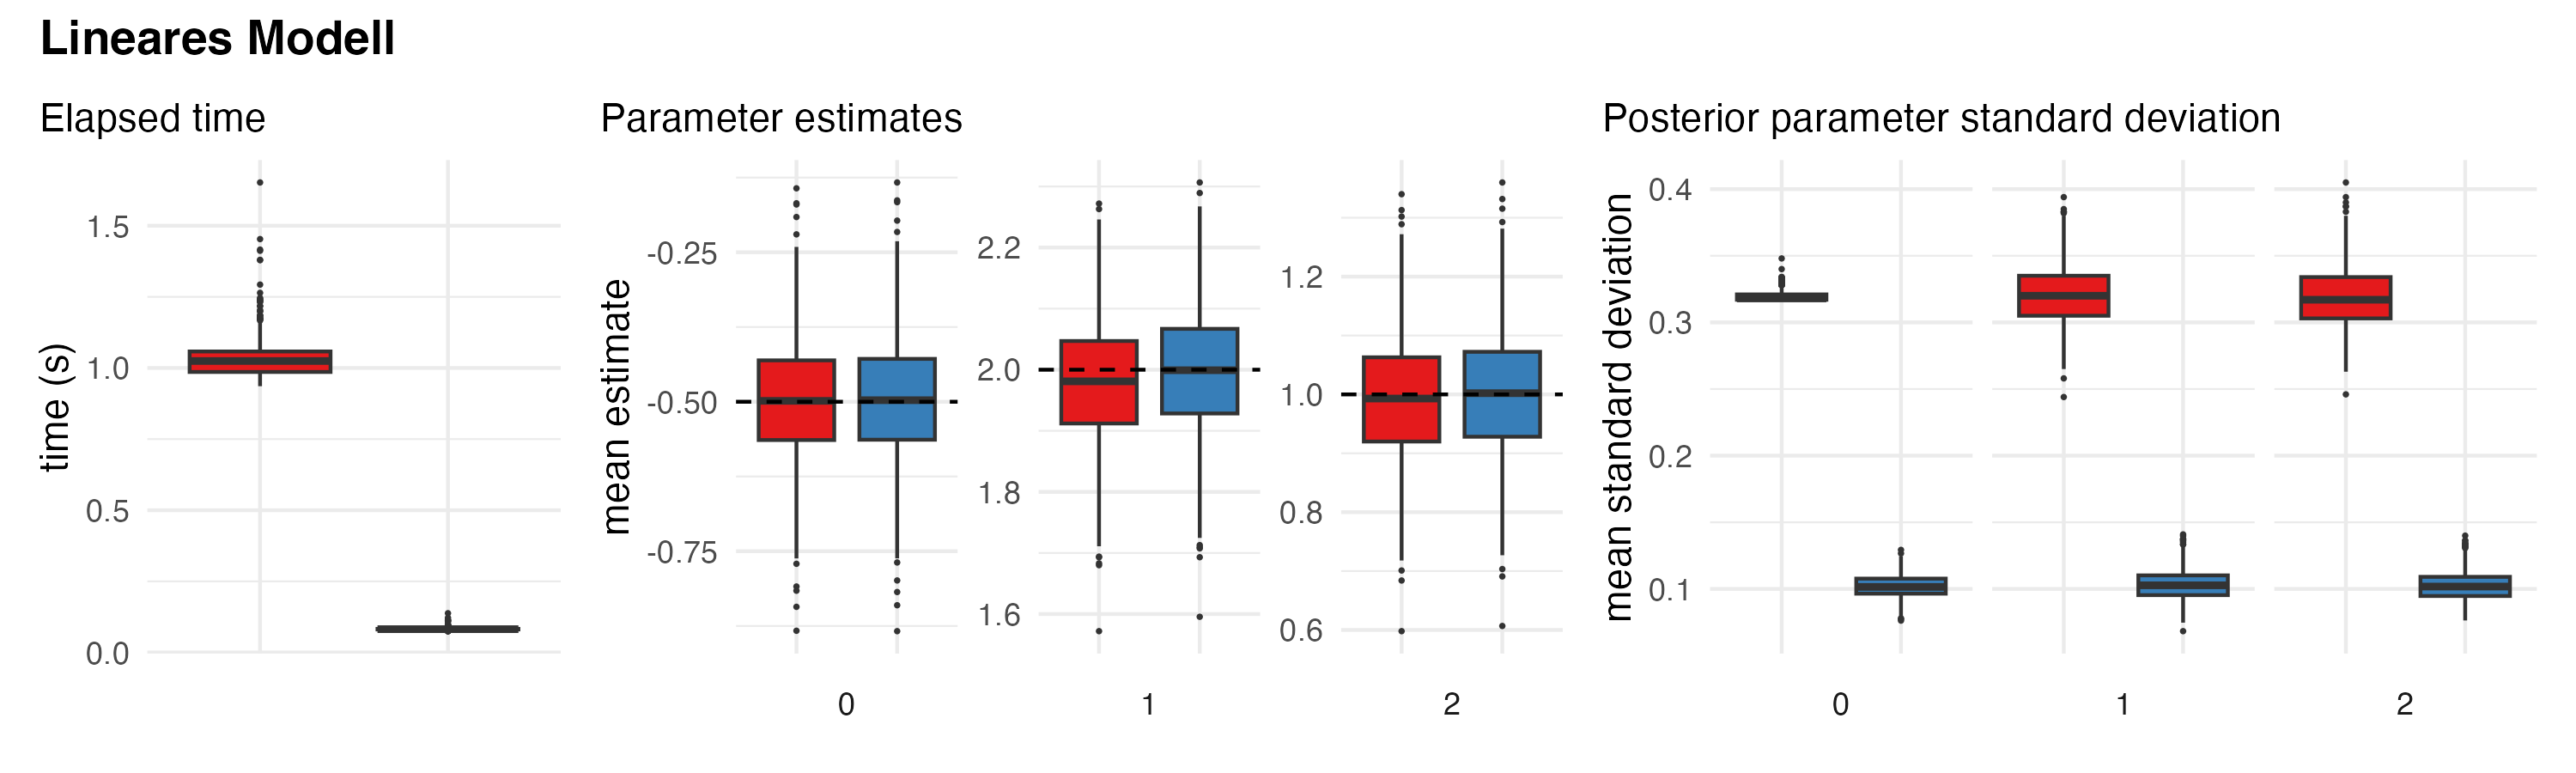
\includegraphics[width=0.85\linewidth,height=\textheight,keepaspectratio]{../figures/approx_plot_regr.png}
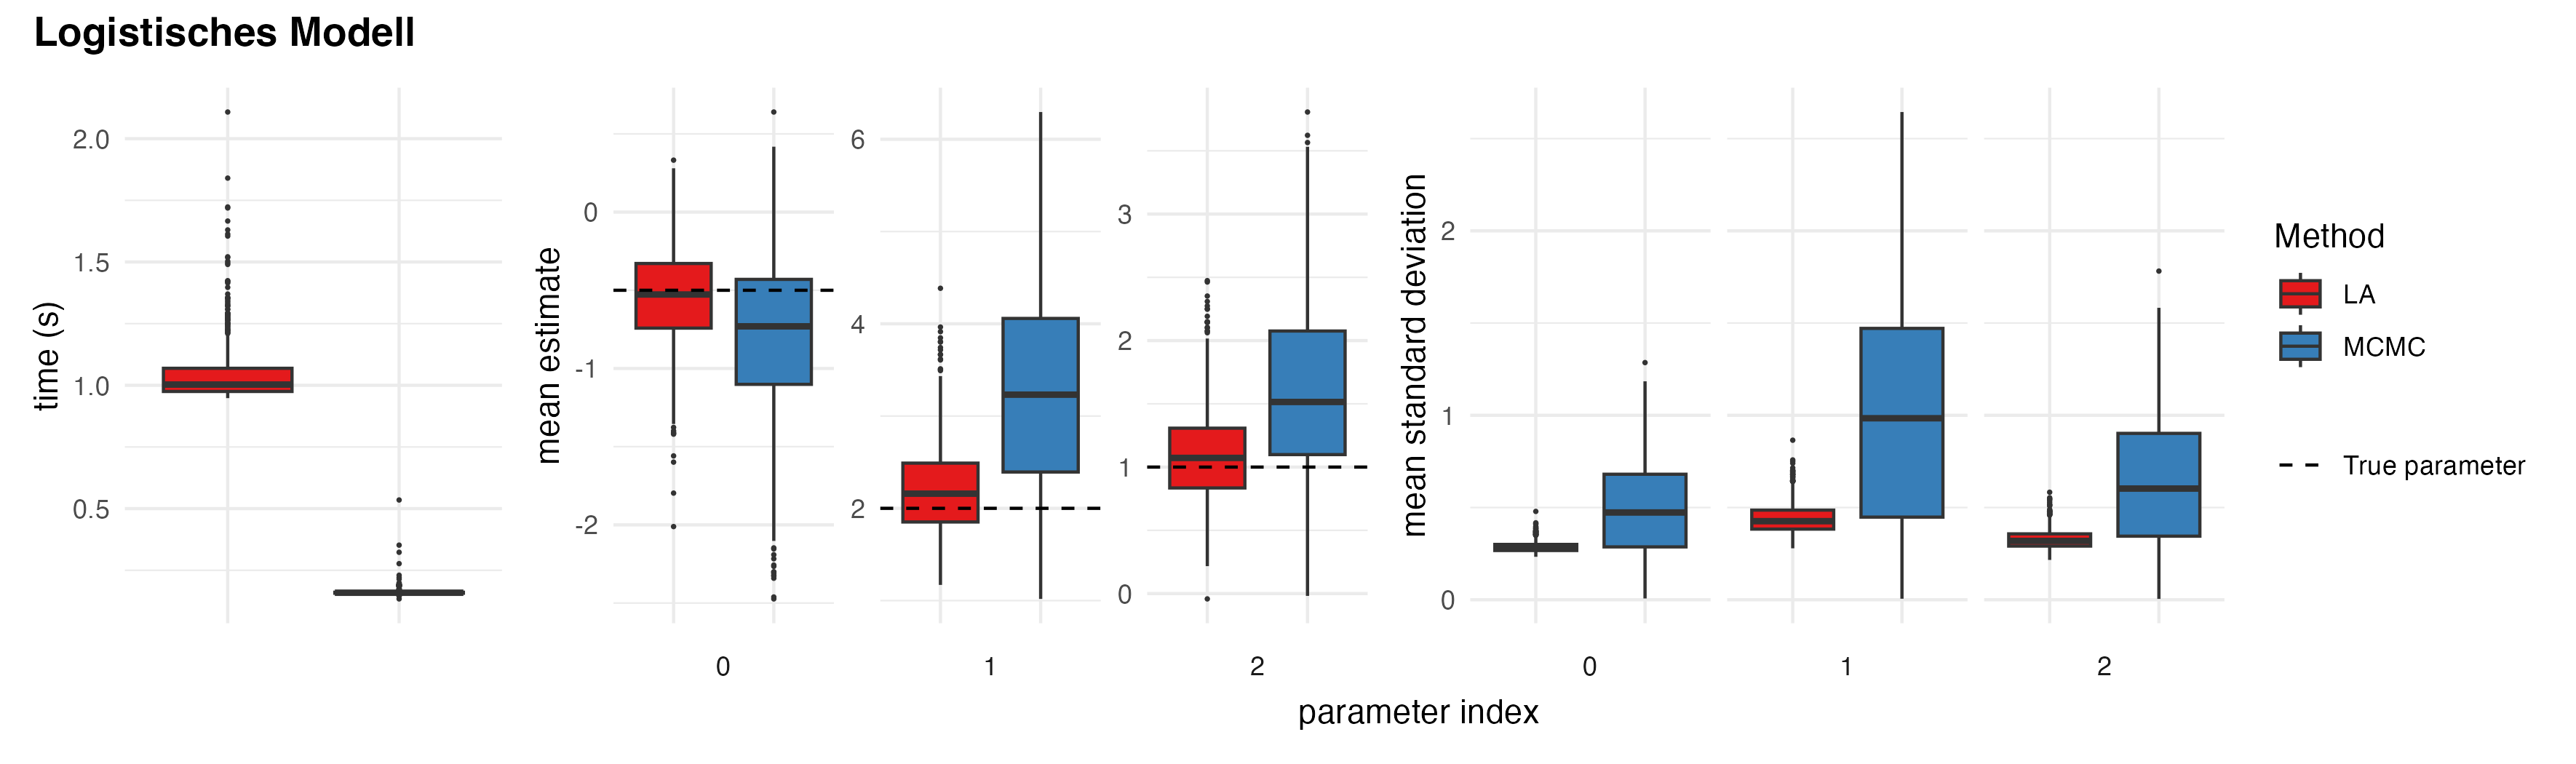
\includegraphics[width=0.97\linewidth,height=\textheight,keepaspectratio]{../figures/approx_plot_class.png}
\end{frame}

\begin{frame}{Vorhersagen mit bayesianischen Modellen}
\protect\phantomsection\label{vorhersagen-mit-bayesianischen-modellen}
Aus der Bayes Regel:
\[p(\by) = \int p(\by, \btheta) d\btheta = \int p(\by \mid \btheta) p(\btheta) d\btheta\]

\begin{block}{Posterior Predictive Distribution}
\protect\phantomsection\label{posterior-predictive-distribution}
\(\to\) Vorhersagen für \(\tX\) im Bayesianischen GLM
\autocite{box_sampling_1980,barbieri_posterior_2015}

\[
p(\ty \mid \by) = \int p(\ty, \btheta \mid \by) d \btheta 
    = \int p(\ty \mid \btheta, \by) p(\btheta) d \btheta
    \overset{\ty \perp \by \mid \btheta}{=}  \int p(\ty \mid \btheta) p(\btheta) d \btheta
\]
\end{block}

Für das bayesianische \textbf{logistische Modell} berechnet man
\[p(\ty = 1 \mid \by)\] mit
\(y_i \in \{0 \text{ (negative)}, 1 \text{ (positive)}\}\)

TODO: Bild
\end{frame}

\begin{frame}{Berechnung der Posterior Predictive Distribution}
\protect\phantomsection\label{berechnung-der-posterior-predictive-distribution}
\textbf{Analytische Berechnung}: z.B. für die NIG-Prior ergibt sich
\[\ty \mid \btheta, \ssd, \by \sim \Tcal(2 \apo, \tX \btheta, \frac{\bpo}{\apo} (\bI + \tX \Sdpo \tX^\top))\]

Alternativ (und viel wichtiger): \textbf{Approximation}

\begin{itemize}
\tightlist
\item
  für Metropolis-Hastings:
  \(p(\ty = 1 \mid \btheta, \by) \approx \frac{1}{K} \sum_{k=1}^{K} \sigma(\tX \btheta^{(k)})\)
\item
  für Laplace Approximation:

  \begin{itemize}
  \item
    LA-approximierte PPD analytisch berechnen:

    \[p(\ty = 1 \mid \btheta, \by) = \int \sigma(\tX \btheta) \Ncal_{\btheta}(\hbtheta_{MAP}, H^{-1} (\hbtheta_{MAP})) \; d \btheta\]
  \item
    Samples
    \(\btheta^{(s)} \sim \Ncal(\hbtheta_{MAP}, H^{-1}(\hbtheta_{MAP}))\)
    mit \(s = 1, \dots, S\) aus der LA-approximierten Parameter
    Posterior ziehen und wie bei Metropolis-Hastings vorgehen
  \end{itemize}
\end{itemize}
\end{frame}

\begin{frame}[fragile]{Literatur Empfehlungen}
\protect\phantomsection\label{literatur-empfehlungen}
\begin{itemize}
\tightlist
\item
  Bayesianische Regression (v.a. für praktische Anwendung):
  \textcite{gelman_bayesian_2013}
\item
  Prior Verteilungen (v.a. Shrinkage): \textcite{van_erp_shrinkage_2019}
  und \textcite{celeux_regularization_2012}
\item
  Software: z.B. \texttt{brms} in \texttt{R}, \texttt{PyMC} in
  \texttt{python}
\end{itemize}
\end{frame}

\section{Referenzen}\label{referenzen}

\section{Anhang}\label{anhang}

\begin{frame}{Herleitung der kojugierten Priori}
\protect\phantomsection\label{herleitung-der-kojugierten-priori}
.
\end{frame}

\begin{frame}{Ergebnisse des Regularisierungsexperiments}
\protect\phantomsection\label{ergebnisse-des-regularisierungsexperiments}
.
\end{frame}

\begin{frame}{Posterior Inference: exakter Metropolis (-Hastings)
Algorithmus}
\protect\phantomsection\label{posterior-inference-exakter-metropolis--hastings-algorithmus}
\begin{enumerate}
\tightlist
\item
  Initialize \(\btheta^{(1)}\)
\item
  For \(k = 1, \dots, K\)

  \begin{enumerate}
  \item
    Draw \(\btheta^{(*)}\) from the \textit{proposal distribution}
    \(q(\btheta^{(*)} \mid \btheta^{(k)})\)
  \item
    calculate the \textit{acceptance probably}

    \[
         \alpha = \min \Bigl(
             1, \frac{
                 p(\btheta^{(*)} \mid \by)\; p(\btheta^{(*)}) \; q(\btheta^{(k)} \mid \btheta^{(*)})}{
                     p(\btheta^{(k)} \mid \by)\; p(\btheta^{(k)}) \; q(\btheta^{(*)} \mid \btheta^{(k)})
                 }
             \Bigr)
     \]
  \item
    Accept or discard the proposal \(\btheta^{(*)}\) (for
    \(u \sim \text{Uni}[0, 1]\))

    \[
     \begin{cases}
             u \le \alpha & \btheta^{(k+1)} = \btheta^{(*)}\\
             u > \alpha & \btheta^{(k+1)} = \btheta^{(k)}\\
     \end{cases}
     \]
  \end{enumerate}
\end{enumerate}

Und z.B. \[
q(\btheta^{(*)} \mid \btheta^{(k)}) \sim \Ncal(\btheta^{(k)} \mid -H^{-1}(\btheta^{(k)}))
\] mit
\(H(\btheta) = \nabla_{\btheta}^2  \log \Bigl(p(\btheta^{(k)} \mid \by)\; p(\btheta^{(k)})\Bigr)\)
\end{frame}

\begin{frame}{Posterior Inference: Mittelwert und Varianz für Laplace
Approximation}
\protect\phantomsection\label{posterior-inference-mittelwert-und-varianz-fuxfcr-laplace-approximation}
Exemplarische Berechnung für ein bayesianisches logistisches Modell mit
der Prior \(\btheta \sim \Ncal(\bnull, \ssd \bI)\):

Es gilt dass mit Laplace Approximation
\(p(\btheta \mid \by) \approx \Ncal(\hbtheta_{MAP}, H^{-1}(\hbtheta_{MAP}))\)
mit

\[
\begin{aligned}
    \hbtheta_{MAP} &= \arg \max_{\btheta} p(\btheta \mid \by)
        \overset{\text{Bayes' rule}}{=} \arg \max_{\btheta} p(\by \mid \btheta) p(\btheta) \; d\btheta  \\
        &= \arg \max_{\btheta} \sumin \log \Bigl( \sigma(y_i \; \bx_i\btheta)\Bigr) - \frac{1}{2 \ssd} \btheta^\top \btheta \\
    H(\btheta) &= - \nabla^2_{\btheta}  \log p (\btheta \mid \by) = \frac{1}{\ssd} \bI + \sumin
    \sigma(y_i \; \bx_i\btheta) \Bigl(1 - \sigma(y_i \; \bx_i\btheta)\Bigr)
        \bx_i \bx_i^\top.
\end{aligned}
\]
\end{frame}

\begin{frame}{Experiment-Setup: Regularisierung}
\protect\phantomsection\label{experiment-setup-regularisierung}
\end{frame}

\begin{frame}{Beispiel 1: Regularisierung in data-sparse Szenarien}
\protect\phantomsection\label{beispiel-1-regularisierung-in-data-sparse-szenarien}
\end{frame}

\begin{frame}{Experiment-Setup: approximate Inference}
\protect\phantomsection\label{experiment-setup-approximate-inference}
.
\end{frame}

\begin{frame}[allowframebreaks]{}
  \bibliographytrue
  \printbibliography[heading=none]
\end{frame}

\end{document}
